\section{Methodology}
\label{section:methodology}
To analyze the new approach for XCS in dynamic scenarios in the following the specific scenario settings (see Section~\ref{subsection:scenario-settings}), the obstacle configurations (see Section~\ref{subsection:scenario-obstacle}) and the implementation of the XCS variants (see Section~\ref{subsection:xcs-variants}) will be discussed.

% Putting all together the properties of the scenario are then compared to the properties of environments without the Markov property (see Section~\ref{subsection:scenario-classification}) and then classified according to the results of the discussion in Section~\ref{subsection:non-markov-environments}.


\subsection{Sensory abilities}

\begin{figure}[ht]
	\subfigure[Sight range]{
  	\label{figure:sight-range}
		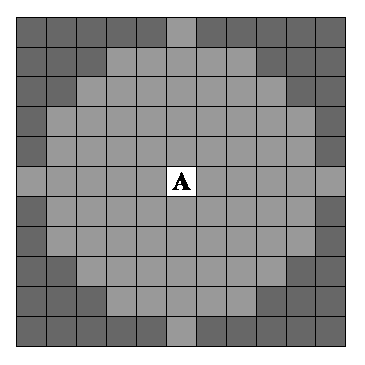
\includegraphics[height=2.62cm]{sight_range.eps}}\hfill
  \subfigure[Observation range]{
  	\label{figure:observation-range}
  	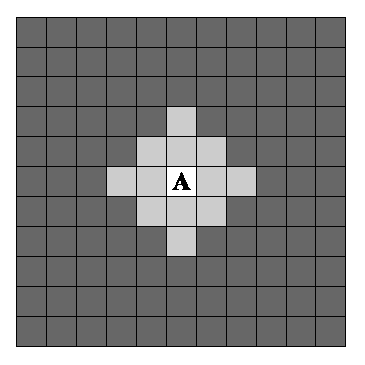
\includegraphics[height=2.62cm]{observation_range.eps}}\hfill
  \subfigure[Example situation]{ % with an agent, trees and food/prey]{
  	\label{figure:example-sight-observation}
  	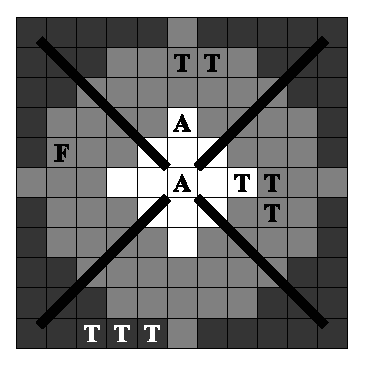
\includegraphics[height=2.62cm]{example_sight_observation.eps}}
  \caption{\mathversion{bold}Sensor ranges of individual agents and an example situation: Obstacles/trees are marked with $T$, prey/food is marked with $F$, predators/agents are marked with $A$, and the observation and sight ranges are marked with light gray and gray color, respectively. Areas, which are out of sight of any predator, are marked with dark gray color.}
  \label{figure:sight-directions}
\end{figure}

\begin{figure}[ht]
	\centerline{
		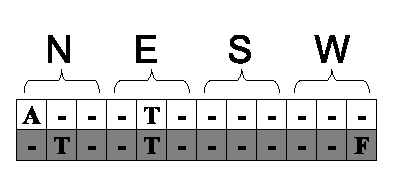
\includegraphics[width=0.2\textwidth]{example_string.eps}
	}
	\caption{\mathversion{bold}Matching sensor data string for central agent in the example, as depicted in Figure~\ref{figure:example-sight-observation}}
	\label{figure:example-string}
\end{figure}

Both, the prey and the predators, have 24 binary sensors that can sense their close environment, but their lines of sight can be blocked by objects. Half of the sensors can detect objects, which are two fields away, while the other half can detect objects up to five fields away, as depicted in Figure~\ref{figure:sight-directions}. % The 12 sensors for each sight range are for the four directions and the three types of objects (prey, other agents and obstacles). An example of a resulting sensor data string is shown in Figure~\ref{figure:example-string}.
Thus, 12 binary-coded sensors are used for both sight and observation range to encode every possible situation, as shown in Figure~\ref{figure:example-string}. Three bits are used to characterize a specific situation (prey, other predators and obstacles) for each direction (north, east, south and west). 

\subsection{Scenario Settings}
\label{subsection:scenario-settings}

The different XCS implementations are tested in a simple predator/prey scenario on a discrete, quadratic and toroidal world consisting of $16 \times 16$ squares. A cell of the two-dimensional grid-world can only be occupied by one agent. 
%One non-learning prey randomly moves over the field while 
Eight adaptive predators follow an observation strategy, i.\,e., they cooperatively have to learn to keep the moving, non-learning prey under observation. Thereby, every predator possesses its own XCS instance. 

The \emph{average} \emph{quality} of the observation task is determined by the amount of time any predator has the prey in its observation range. It is calculated by averaging the qualities of 100 experiments, each consisting of 10 runs. The \emph{continuous average quality} denotes the average quality of the last 2\,000 steps only. In detail, each run consists of 2\,000 steps, after which the scenario is reset. The individual learning experiences of the agents are saved between each run, but not between each experiment. In each time step, each predator can only move to one of the four neighboring fields, while the prey can move two fields, which allows for a faster movement. In addition, there are obstacles on the field and any movement to an occupied field fails (without any further consequences). 

The simulation is conducted in discrete time. At every time step, the prey and the predators gather sensor data and decide their next actions. Then, all actions of all agents are executed in a random sequence. Since the prey can move two fields per each simulation step, it gathers new sensor data after the first step. If the prey is surrounded by predators in all four neighboring directions, it will jump to a random free field nearby, which basically means a restart of the simulation. Experiments have shown that this random jumping strategy only happens very seldom, i.\,e., it does not significantly alter the simulation results.


\subsection{Scenario Configurations}
\label{subsection:scenario-obstacle}

\begin{figure}[ht]
	\subfigure[\emph{Pillar sce\-nar\-io}]{
		\label{figure:pillar-scenario}
		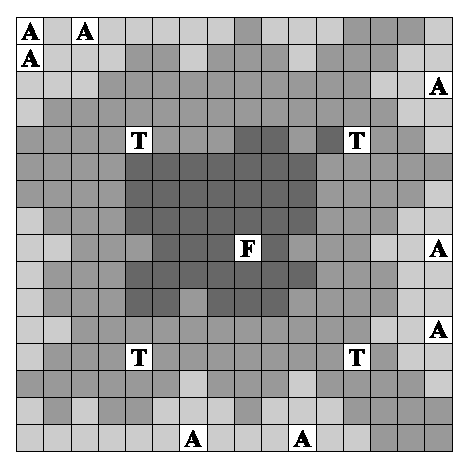
\includegraphics[height=2.62cm]{pillar_scenario.eps}}\hfill
  \subfigure[\emph{Random sce\-nar\-io}]{
  	\label{figure:random-scenario}
  	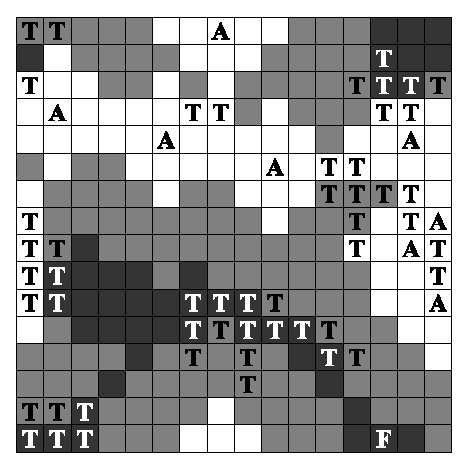
\includegraphics[height=2.62cm]{random_scenario.eps}}\hfill
  \subfigure[\emph{Difficult sce\-nar\-io}]{
  	\label{figure:difficult-scenario}
  	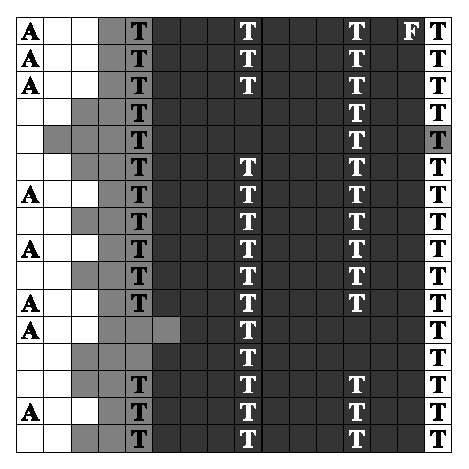
\includegraphics[height=2.62cm]{difficult_scenario.eps}}
  % \caption{\mathversion{bold}Sample start configurations for the three different scenarios: Obstacles/trees are marked with $T$, prey/food is marked with $F$, predators/agents are marked with $A$, and the observation and sight ranges are marked with light gray and gray color, respectively. Areas, which are out of sight of any predator, are marked with dark gray color.}
  \caption{Sample start configurations for the three different scenarios}
  \label{figure:scenarios}
\end{figure}

Three different configurations of obstacles (trees) and star\-ting positions of prey and predators have thoroughly been tested. In the \emph{pillar scenario} (see Figure~\ref{figure:pillar-scenario}), four obstacles are arranged in equal distance to each other, the prey starts in the middle of the whole field, and the predators start randomly positioned along the borders. The idea of this scenario has been to use a minimal number of obstacles while still giving the agents some points of orientation.
In the second scenario, the \emph{random scenario} (see Figure~\ref{figure:random-scenario}), several obstacles are randomly distributed on the whole grid with a certain tendency to build connected structures. In both scenarios, the \emph{pillar scenario} and the \emph{random scenario}, two kinds of prey implementations have been evaluated. The first one tries to move away from predators (the so-called \emph{predator-evading prey}), while the second one tries to evade collisions with obstacles (the \emph{obstacle-evading prey}). % Both types of a prey randomly move whether predators or obstacles are in the local neighborhood. % walk strategy as well, but tries to evade collisions with obstacles.
If there are several alternatives, both types will move into a random direction, in which the prey does not see predators or obstacles, respectively.
The third scenario, the \emph{difficult scenario} (see Figure~\ref{figure:difficult-scenario}), provides a simple maze with several walls and small openings. Predators start on the left and have to find the openings that lead them into the direction of the prey, while the prey only stays in the area on the right 
by moving northward only and evading an agent if necessary. 
%and continuously moves northward for two fields (or will jump to a free field nearby, if the direct path is blocked in northern direction). 
As the prey ignores sensory information it will be referred to as the \emph{blinded prey}. 
While this makes the actual observation task easier, the point of this scenario was to test if the agents are still able to find a way through a maze.
%possessed the capabilities of XCS to 

\subsection{XCS Variants}
\label{subsection:xcs-variants}



All XCS variants that are here investigated have in common that the corresponding scenario will not be restarted, if a positive reward is attained (as it appears in the standard XCS implementation). The first variant, which will be referred to as \textbf{XCS~(obs)}, is equal to the standard implementation in all other implementation aspects, i.\,e., the global goal is equivalent to the local goal and predators act according to the \emph{selfish behavior (observation range)} strategy (see Section~\ref{subsection:environment-reward-function}). Including more sensor information to the predators' behavior by using the \emph{selfish behavior (sight range)} strategy is denoted with \textbf{XCS~(sight)}. Combining this variant with the event handling mechanism (see Section~\ref{subsection:events}) and using a reward distribution based on these generated events (see Section~\ref{subsection:reward-distribution}) is referred by \textbf{eventXCS} as a third variant. Replacing also the selection strategy \emph{best selection} (see Section~\ref{section:learning-classifier-systems}) with \emph{tournament selection} (with $p = 0.84$, see~\cite{Butz2003}) results in an XCS variant, as denoted with \textbf{eventXCS~(ts)}. Finally, the usage of the \emph{cooperative behavior} strategy is marked with \textbf{eventXCS~(coop,~ts)}.



